\documentclass[aspectratio=169]{beamer}
\usepackage[utf8]{inputenc}

% design
\usetheme{CambridgeUS}
\usecolortheme{beaver}
\setbeamertemplate{itemize items}[square]
\usenavigationsymbolstemplate{\beamertemplatenavigationsymbolsempty}
\definecolor{darkred}{rgb}{0.8,0,0}
\colorlet{grey1}{gray!10!white} % I think = RGB 0.95 0.95 0.95
\colorlet{grey2}{gray!60!white} % I think = RGB 0.7 0.7 0.7
\setbeamertemplate{enumerate item}{\color{darkred}\insertenumlabel.}
\setbeamertemplate{itemize item}{\color{darkred}$\blacktriangleright$}
\setlength{\tabcolsep}{12pt}
\setbeamercolor{block title}{fg=darkred}

% bibliography
%\usepackage[backend=biber, style=authortitle]{biblatex}
\usepackage{natbib}
\usepackage{har2nat}
\bibliographystyle{unsrt}
%\addbibresource{../../smc.bib}
\usepackage{bibentry}
\nobibliography*

% tikz
\usepackage{tikz}
\usetikzlibrary{positioning}

% maths
\usepackage{amsmath}
\usepackage{amssymb}
\usepackage{amsfonts}
\usepackage{amsthm}
\theoremstyle{definition}
\newtheorem{defn}{Definition}

% useful math symbols
\newcommand{\PR}{\mathbb{P}}
\newcommand{\E}{\mathbb{E}}
\newcommand{\V}{\operatorname{Var}}
\newcommand{\eqdist}{\overset{d}{=}}
\newcommand{\I}[1]{\mathbb{I}\{#1\}}
\newcommand{\Ntoinfty}{\overset{N\to\infty}{\longrightarrow}}
\newcommand{\limNtoinfty}{\underset{N\to\infty}{\lim}}
\newcommand\indep{\protect\mathpalette{\protect\independenT}{\perp}}
\def\independenT#1#2{\mathrel{\rlap{$#1#2$}\mkern2mu{#1#2}}}

% distributions
\newcommand{\N}{\mathcal{N}}
\newcommand{\Cat}{\operatorname{Categorical}}
\newcommand{\Unif}{\operatorname{Uniform}}
\newcommand{\Mn}{\operatorname{Multinomial}}
\newcommand{\Bin}{\operatorname{Binomial}}

% project-specific commands
\newcommand{\F}{\mathcal{F}_{t-1}}
%\newcommand{\vt}[2][t]{v_{#1}^{(#2)}}
\newcommand{\vt}[1]{v_{#1}}
%\newcommand{\wt}[2][t]{w_{#1}^{(#2)}}
\newcommand{\wt}[1]{w_{#1}}
%\newcommand{\wbar}[2][t]{\bar{w}_{#1}^{(#2)}}
%\newcommand{\vttilde}[2][t]{\tilde{v}_{#1}^{(#2)}}

\title[SMC genealogies]{Genealogies of sequential Monte Carlo algorithms}
\author{Suzie Brown}
\date{27 October 2020} 

\begin{document}
\begin{frame}
\maketitle
\end{frame}


\begin{frame}{Outline}
\begin{enumerate}
\item Sequential Monte Carlo
\item Resampling and degeneracy
\item Genealogies
\end{enumerate}
\end{frame}


\begin{frame}{Sequential Monte Carlo}
\begin{itemize}
\item Want to sample from a sequence of intractable target distributions
\item Typical setting: dimension of target increases in time, or strong dependence between consecutive targets (so MCMC is impractical)
\item SMC can obtain exact draws, and thus approximate expectations
\end{itemize}

%%% NOTES
% Typically the sequence is indexed by time
% Run-time is linear in number of dimensions, cf MCMC
% Dependence between consecutive targets is a help rather than a hindrance, cf MCMC
% Inference can be done on-line

\end{frame}


\begin{frame}{State space models}
\begin{columns}
\begin{column}{0.45\textwidth}
\begin{center}
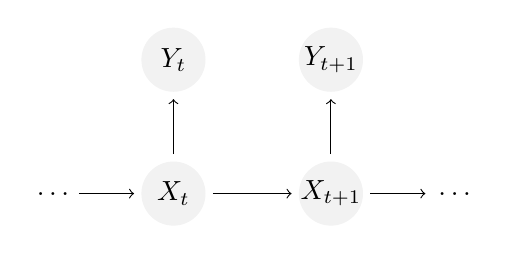
\begin{tikzpicture}
\filldraw[grey1] (0,0) circle (0.4);
\filldraw[grey1] (0,1.7) circle (0.4);
\filldraw[grey1] (2,0) circle (0.4);
\filldraw[grey1] (2,1.7) circle (0.4);
\node at (2,1.7) {$Y_{t+1}$};
\node at (2,0) {$X_{t+1}$};
\node at (0,1.7) {$Y_{t}$};
\node at (0,0) {$X_{t}$};
\node at (-1.5,0) {$\dots$};
\node at (3.6,0) {$\dots$};
\draw[->] (-1.2,0)--(-0.5,0);
\draw[->] (0.5,0)--(1.5,0);
\draw[->] (2.5,0)--(3.2,0); 
\draw[->] (0,0.5)--(0,1.2);
\draw[->] (2,0.5)--(2,1.2);
\end{tikzpicture}
\end{center}
\begin{align*}
& X_0 \sim \mu(\cdot) \\
& X_{t+1} \mid (X_t = x_t) \sim f_t(\cdot | x_t)\\
& Y_t \mid (X_t = x_t) \sim g_t(\cdot | x_t)
\end{align*}
\end{column}
\begin{column}{0.45\textwidth}
May want to infer ($t<T$):

\renewcommand{\arraystretch}{1.5}
\begin{tabular}{l l}
$p(x_{1:T} \mid y_{1:t})$ & ``prediction'' \\
$p(x_{1:t} \mid y_{1:t})$ & ``filtering'' \\
$p(x_{1:t} \mid y_{1:T})$ & ``smoothing''
\end{tabular}
\end{column}
\end{columns}

%%% NOTES
% Flexible class of models much used in applications
% Helpful for illustrating SMC
%-
% X = hidden states we want to infer
% Y = (noisy) observations
%-
% Intractable except in a few special cases
% Examples: stochastic volatility, target tracking
\end{frame}

%\begin{frame}{Example: sleep monitoring}
%\begin{itemize}
%\item $X_t$ encodes the patient's state awake/asleep
%\item $Y_t$ is a vector of observations, say heart rate and body temperature
%\item Want to infer how well the patient slept over the whole night $\rightarrow$ smoothing
%\end{itemize}
%\centering
%\includegraphics[width=0.8\textwidth]{ssm_ex_2.jpg}
%
%%%% NOTES
%% The example is in continuous time, but can easily imagine discrete observations (in fact only possible to get discrete obs!)
%% Model X as a Markov process with two states (so just need to choose switching rates/probabilities)
%% Also have some model for how temperature and heart rate vary with sleep
%% Actually this is a terrible example because it hardly makes sense to assume that Y_{t+1} depends on Y_t only via X...
%\end{frame}

\begin{frame}{Importance Sampling}
\centering

\end{frame}


%%%----------------- old slides below here ------------------

%%% NOTES
% if you were here two weeks ago Francesca gave an intro to SMC - mine will be quite different (motivational & vague)
% genealogies is the part I'm primarily working on



\begin{frame}{Sequential Monte Carlo}{Illustration}
\begin{center}
\resizebox{0.95\textwidth}{!}{%
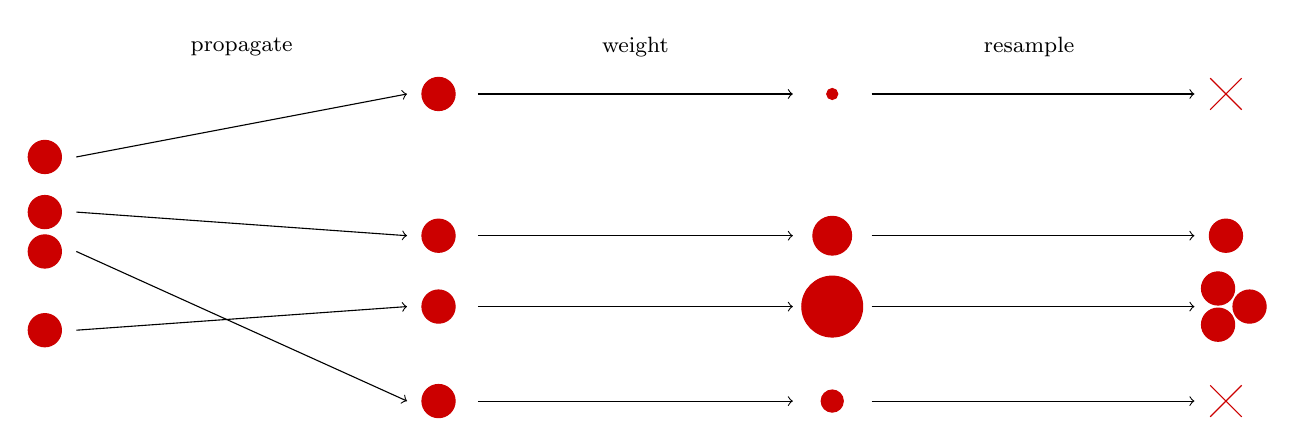
\begin{tikzpicture}
\filldraw[darkred] (0,0) circle (6pt);
\filldraw[darkred] (0,1) circle (6pt);
\filldraw[darkred] (0,1.5) circle (6pt);
\filldraw[darkred] (0,2.2) circle (6pt);

\draw[->] (0.4,2.2) -- (4.6,3);
\draw[->] (0.4,1.5) -- (4.6,1.2);
\draw[->] (0.4,1) -- (4.6,-0.9);
\draw[->] (0.4,0) -- (4.6,0.3);

\filldraw[darkred] (5,0.3) circle (6pt);
\filldraw[darkred] (5,-0.9) circle (6pt);
\filldraw[darkred] (5,1.2) circle (6pt);
\filldraw[darkred] (5,3) circle (6pt);

\draw[->] (5.5,3) -- (9.5,3);
\draw[->] (5.5,1.2) -- (9.5,1.2);
\draw[->] (5.5,-0.9) -- (9.5,-0.9);
\draw[->] (5.5,0.3) -- (9.5,0.3);

\filldraw[darkred] (10,0.3) circle (11pt);
\filldraw[darkred] (10,-0.9) circle (4pt);
\filldraw[darkred] (10,1.2) circle (7pt);
\filldraw[darkred] (10,3) circle (2pt);

\draw[->] (10.5,1.2) -- (14.6,1.2);
\draw[->] (10.5,0.3) -- (14.6,0.3);
\draw[->] (10.5,-0.9) -- (14.6,-0.9);
\draw[->] (10.5,3) -- (14.6,3);

\filldraw[darkred] (15.3,0.3) circle (6pt);
\filldraw[darkred] (14.9,0.53) circle (6pt);
\filldraw[darkred] (14.9,0.07) circle (6pt);
\filldraw[darkred] (15,1.2) circle (6pt);

\draw[darkred] (14.8,3.2) -- (15.2, 2.8);
\draw[darkred] (14.8,2.8) -- (15.2, 3.2);
\draw[darkred] (14.8,-0.7) -- (15.2, -1.1);
\draw[darkred] (14.8,-1.1) -- (15.2, -0.7);

\node at (2.5,3.6) {\footnotesize{propagate}};
\node at (7.5,3.6) {\footnotesize{weight}};
\node at (12.5,3.6) {\footnotesize{resample}};
\end{tikzpicture}
}
\end{center}
\end{frame}



\begin{frame}{Resampling and Genealogies}
\begin{columns}
\begin{column}{0.45\textwidth}
\begin{itemize}
\item Resampling creates a genealogy (family tree) of particles
\item Properties of the genealogy affect performance of the SMC algorithm
\item Different resampling schemes give different forms of genealogies
\item Basic quantity for analysing genealogies is the pair coalescence probability
\end{itemize}
\end{column}
\begin{column}{0.45\textwidth}
%\includegraphics[width=\textwidth]{eg_WF.pdf}
\end{column}
\end{columns}
\end{frame}


\begin{frame}{Coalescence Probability}{Definition}
The probability that a randomly chosen pair of particles at generation $t$ share a common ancestor at generation $(t-1)$
\begin{equation*}
c_N = \frac{1}{N(N-1)} \sum_{i=1}^N \vt{i}(\vt{i}-1)
\end{equation*}

%%% NOTES
% N(N-1) is the number of pairs from which we choose uniformly
% the sum is over all possible parents that could be a common ancestor for the pair
% v_i(v_i-1) =0 if that parent had only one child, and is the number of ways this pair could be chosen from the i^th parent's offspring.
\end{frame}


\begin{frame}{Coalescence Probability}{Example}
Consider the case where we have only two particles ($N=2$)
\begin{equation*}
c_2 = \frac{1}{2}\left[ \vt{1}(\vt{1}-1) + \vt{2}(\vt{2}-1)\right]
\end{equation*}
The expectation of $c_2$ conditional on knowing the weights $(\wt{1}, \wt{2})$ is
\begin{align*}
c_2 &= \frac{1}{2} \E[\vt{1}(\vt{1}-1) \mid \wt{1:2}] + \frac{1}{2} \E[\vt{2}(\vt{2}-1) \mid \wt{1:2}] \\
&= \PR[\vt{1}=2 \mid \wt{1:2}] + \PR[\vt{2}=2 \mid \wt{1:2}]
\end{align*}

%%% NOTES
% The only possible values of v_i are 0,1,2. 
% If 0,1 then v_i(v_i-1)=0
% If 2 then v_i(v_i-1)=2
% write as E[ 2* I{v_i=2} |w] to get the last line.
%
% Multinomial: w_1^2 + w_2^2
% Residual-mn: (2w_1 -1)I{w_1>0.5} + (2w_2 -1)I{w_2>0.5}
\end{frame}


\begin{frame}{Coalescence Probability}{Example}
\centering
%\includegraphics[width=0.7\textwidth]{EcN_mn_res_n2.pdf}

%%% NOTES
% (N=2) For all weight vectors, coalescence rate is lower with residual-multinomial than with multinomial
% Stratified & systematic resampling have the same curve as residual
% More interesting in higher dimensions, but difficult to plot!
% (Also proved dominance of res-mn over mn also for N=3 but no general-N proof yet)
% NB: slow coalescence is good because we keep distinct samples for longer
\end{frame}


\begin{frame}
\begin{itemize}
\item We proved that asymptotically (as $N\to\infty$) residual resampling dominates multinomial in terms of expected coalescence probability
\item We also proved it in cases $N=2$ and $N=3$
\pause
\item We conjecture that it holds for all finite $N$ too
\item It just remains to prove it for $N=4,5,\dots$
\pause
\item We proved that systematic resampling (and some others) dominate multinomial in expected coalescence probability, for all $N$.
\end{itemize}
%%% NOTES 
% Everything is conditional on weights
% Probability -> rate in asymptotic regime
% "Some others" means all stochastic-rounding-based schemes, for those who know what that means
\end{frame}


\begin{frame}
\centering
THE END
\end{frame}
\end{document}